\documentclass[onecolumn, aps, nofootinbib, prd, preprint, floats, floatfix, amsmath, amssymb, superscriptaddress, preprintnumbers]{revtex4-1}
\PassOptionsToPackage{dvipsnames}{xcolor}
\usepackage{slashed}
\usepackage{graphicx}
\usepackage{subcaption}
\usepackage{dcolumn}
\usepackage{bm}
\usepackage{amssymb}
\usepackage{tikz-feynman}
%\usepackage{xcolor}
\usepackage[utf8]{inputenc}
% \usepackage[OT1]{fontenc}
\usepackage{yfonts,amsmath,amsthm,amsfonts,amssymb,amscd, ulem}
\usepackage{enumerate}
\usepackage{fancyhdr}
\usepackage{mathtools}
\usepackage{mathrsfs}
\usepackage{cancel}
\usepackage{slashed}
\usepackage{bigints}
\usepackage[flushleft]{threeparttable}
\usepackage[colorlinks=true, citecolor=purple, linkcolor=blue]{hyperref}
\usepackage{url}
\usepackage{makecell,booktabs}
\usepackage{braket}
\usepackage{relsize}
\usepackage{multirow}
\usepackage{verbatim}
\usepackage{txfonts}
\usepackage{slashed}
\usepackage{upgreek}
\usepackage{extarrows}
\usepackage{array}
\usepackage{appendix}
\usepackage[T1]{fontenc}
\usepackage{setspace}
\usepackage{subcaption}
\newcommand{\GJH}[1]{\textcolor{blue} {GJH: #1}}
\newcommand{\jl}[1]{\textcolor{orange} {jl: #1}}
\newcommand{\WXP}[1]{\textcolor{purple} {WXP: #1}}
\newcommand{\zb}[1]{{\color{blue} {#1}}}
\usepackage{xcolor}
\definecolor{c1}{HTML}{1bd1a5}
\newcommand{\pch}[1]{\textcolor{c1} {PCH: #1}}
\usepackage{graphicx}   % 引入图片
\usepackage{caption}    % 总 caption 支持
\usepackage{subcaption} % 子图支持
\usepackage{subcaption}
\usepackage{cleveref}

\begin{document}

\title{Axial $U(1)_{L_\mu-L_\tau}$ Vector Boson Model Building and I}
\author{Jia Liu}
\date{May 2026}


\maketitle
\tableofcontents

\section{Introduction}

\section{Model Setup}
\label{sec:model-setup}



We extend the SM gauge group by \(G_{\rm SM}\times U_A(1)'_{L_\mu-L_\tau}\). The axial \(L_\mu-L_\tau\) assignment is
\[
Q(L_\mu)=-Q(\mu_R)=Q_\ell,\qquad
Q(L_\tau)=-Q(\tau_R)=-Q_\ell ,
\]
with the electron sector neutral. We also introduce a complex scalar singlet \(S\) with \(Q_S=2Q_\ell\). Its VEV breaks \(U_A(1)'_{L_\mu-L_\tau}\) and supplies the charge insertion needed to generate the charged-lepton masses. The field content is summarized in Table~\ref{tab:charge-assignment}.

Although each generation is individually chiral under \(U_A(1)'_{L_\mu-L_\tau}\), the triangle anomalies cancel exactly between the \(\mu\) and \(\tau\) sectors. For example, including the \(SU(2)_L\) multiplicity and subtracting the right-handed contribution, \(\mathcal{A}_{[U_A(1)'_{L_\mu-L_\tau}]^3} \propto 2(+1)^3-(-1)^3+2(-1)^3-(+1)^3=0\), and the mixed gravitational anomaly cancels in the same way.
\begin{table}[htbp]
    \centering
    \begin{tabular}{cccc}
    \hline
    Field & $SU(2)_L$ & $U(1)_Y$ & $U_A(1)'_{L_\mu-L_\tau}$ \\
    \hline
    $L_{\mu}=\left(\nu_{\mu}, \mu_L\right)^T$ & $\mathbf{2}$ & $-1 / 2$ & $Q_{\ell}$ \\
    \hline
    $\mu_R$ & $\mathbf{1}$ & -1 & $-Q_\ell$ \\
    \hline
    $E_\mu\left(E_{\mu L}, E_{\mu R}\right)$ & $\mathbf{1}$ & -1 & $Q_\ell$\\
    \hline
    $L_{\tau}=\left(\nu_{\tau}, \tau_L\right)^T$ & $\mathbf{2}$ & $-1 / 2$ & $-Q_\ell$ \\
    \hline
    $\tau_R$ & $\mathbf{1}$ & -1 & $Q_\ell$ \\
    \hline
    $E_\tau\left(E_{\tau L}, E_{\tau R}\right)$ & $\mathbf{1}$ & -1 & -$Q_\ell$\\
    \hline
    $H$ & $\mathbf{2}$ & $1 / 2$ & 0 \\
    $S$ & $\mathbf{1}$ & 0 & $Q_S=2Q_\ell$\\
    \hline
    \end{tabular}
    \caption{Field content and \(U_A(1)'_{L_\mu-L_\tau}\) charge assignment for the axial \(L_\mu-L_\tau\) construction. The electron sector is neutral under \(U_A(1)'_{L_\mu-L_\tau}\).}
    \label{tab:charge-assignment}
\end{table}

\subsection{Lagrangian and Mass Generation}

The ordinary diagonal SM Yukawa operator \(\bar L_\ell H\ell_R\) is forbidden. For the muon, for instance, \(Q(\bar L_\mu)+Q(\mu_R)=-Q_\ell-Q_\ell=-2Q_\ell\). The leading gauge-invariant diagonal mass operators are therefore dimension five:
\begin{equation}
    \mathcal{L}_{\text{5-d}} =
    -\frac{c_\mu}{\Lambda} S\,\bar{L}_\mu H\mu_R
    -\frac{c_\tau}{\Lambda} S^*\,\bar{L}_\tau H\tau_R
    +h.c.,
\end{equation}
where \(Q_S=2Q_\ell\) compensates the chiral charge mismatch. A simple renormalizable origin is obtained by introducing the vector-like charged leptons \(E_\mu\) and \(E_\tau\) listed in Table~\ref{tab:charge-assignment}. The relevant UV Lagrangian is
\begin{equation}
\begin{aligned}
\mathcal{L}_{UV}\supset&
-y_\mu \bar L_\mu H E_{\mu R}
-\lambda_\mu S\,\bar E_{\mu L}\mu_R
-M_{E\mu}\bar E_{\mu L}E_{\mu R}\\
&
-y_\tau \bar L_\tau H E_{\tau R}
-\lambda_\tau S^*\,\bar E_{\tau L}\tau_R
-M_{E\tau}\bar E_{\tau L}E_{\tau R}
+h.c. .
\end{aligned}
\end{equation}
Integrating out the heavy fields at the scale \(M_E\simeq\Lambda\) yields the effective dimension-five operators above. After electroweak and \(U_A(1)'_{L_\mu-L_\tau}\) breaking, and before allowing direct \(\mu\)--\(\tau\) flavor mixing, the charged-lepton mass matrix is
\begin{equation}
\mathcal{L}_m=-
\begin{pmatrix}
	\overline{\ell^{\mu}_L},  &
	\overline{E^\mu_L}, &
	\overline{\ell^\tau_L}, &
	\overline{E^\tau_L}
\end{pmatrix}
\begin{pmatrix}
	0 & y_{\mu}v/\sqrt2  & 0 & 0 \\
	\lambda_\mu v_S/\sqrt2 & M_{E\mu} & 0 & 0\\
	0 & 0 & 0 & y_{\tau}v/\sqrt2\\
    0 & 0 &  \lambda_\tau v_S/\sqrt2 & M_{E\tau}
\end{pmatrix}
\begin{pmatrix}
	\ell^{\mu}_R \\
	E^\mu_R \\
	  \ell^\tau_R \\
	  E^\tau_R \\
\end{pmatrix}
+h.c. .
\label{eq:4by4-mass-no-mutau}
\end{equation}
Here the factors of $1/\sqrt2$ multiply only the entries generated by scalar VEVs; the vector-like masses $M_{E\ell}$ are bare masses.

Gauge invariance also allows an off-diagonal SM-Higgs Yukawa interaction,
\begin{equation}
    \mathcal{L}\supset y_{\mu\tau} (\bar{L}_{\mu}H \tau_R + \bar{L}_{\tau}H \mu_R)+h.c.
\end{equation}
If this term is present, the mass matrix becomes
\begin{equation}
\mathcal{L}_m=-
\begin{pmatrix}
	\overline{\ell^{\mu}_L},  &
	\overline{E^\mu_L}, &
	\overline{\ell^\tau_L}, &
	\overline{E^\tau_L}
\end{pmatrix}
\begin{pmatrix}
	0 & y_{\mu}v/\sqrt2  & y_{\mu\tau}v/\sqrt2 & 0 \\
	\lambda_\mu v_S/\sqrt2 & M_{E\mu} & 0 & 0\\
	y_{\mu\tau}v/\sqrt2 & 0 & 0 & y_{\tau}v/\sqrt2\\
    0 & 0 &  \lambda_\tau v_S/\sqrt2 & M_{E\tau}
\end{pmatrix}
\begin{pmatrix}
	\ell^{\mu}_R \\
	E^\mu_R \\
	  \ell^\tau_R \\
	  E^\tau_R \\
\end{pmatrix}
+h.c. .
\label{eq:4by4-mass-mutau}
\end{equation}
In the phenomenological analysis below we take \(y_{\mu\tau}=0\) as the benchmark flavor limit. This keeps the light charged leptons aligned with the flavor labels used in the trident, pion, beam-dump, and muon-collider calculations. Nonzero \(y_{\mu\tau}\) is a consistent deformation, but then the physical \(A'\) currents should be rotated by the full \(4\times4\) diagonalization matrices and charged-lepton-flavor observables must be included.

In unitary gauge the scalar fields are written as
\begin{equation}
    H = \frac{1}{\sqrt{2}} \begin{pmatrix} 0 \\ v + h_0 \end{pmatrix}, \quad S = \frac{1}{\sqrt{2}} (v_S + s_0)
\end{equation}
Upon spontaneous symmetry breaking, the \(A'\) mass follows from the kinetic term \(|D_\alpha S|^2\):
\begin{equation}
    m_{A'} = |Q_S| g_S v_S = 2 |Q_\ell| g_S v_S
    \equiv 2|g_X|v_S,\qquad g_X\equiv g_SQ_\ell .
\end{equation}
The corresponding effective charged-lepton mass from the dimension-five operator is
\begin{equation}
    m_\ell = \frac{c_\ell v v_S}{2\Lambda}
\end{equation}
The portal interaction \(\lambda_{SH}(S^* S)(H^\dagger H)\) mixes the neutral CP-even scalars. For the usual two-field potential normalization, the mixing angle satisfies
\begin{equation}
    \tan 2\alpha = \frac{\lambda_{SH} v v_S}{\lambda_S v_S^2 - \lambda v^2}
\end{equation}
With the same field ordering as in Eq.~\eqref{eq:4by4-mass-mutau}, the complete CP-even scalar Yukawa interactions before diagonalizing the charged leptons are
\begin{equation}
\mathcal{L}_{h_0,s_0}
=-\overline{\Psi_L}\left(h_0\,Y_H+s_0\,Y_S\right)\Psi_R+h.c.,
\qquad
\Psi_{L,R}=
\begin{pmatrix}
\ell^\mu\\ E^\mu\\ \ell^\tau\\ E^\tau
\end{pmatrix}_{L,R}.
\label{eq:full-scalar-yukawa-gauge}
\end{equation}
For the mass matrix without the optional $\mu$--$\tau$ entry,
\begin{equation}
Y_H=\frac{1}{\sqrt2}
\begin{pmatrix}
0&y_\mu&0&0\\
0&0&0&0\\
0&0&0&y_\tau\\
0&0&0&0
\end{pmatrix},
\qquad
Y_S=\frac{1}{\sqrt2}
\begin{pmatrix}
0&0&0&0\\
\lambda_\mu&0&0&0\\
0&0&0&0\\
0&0&\lambda_\tau&0
\end{pmatrix}.
\label{eq:scalar-yukawa-no-mutau}
\end{equation}
If the allowed $y_{\mu\tau}$ term in Eq.~\eqref{eq:4by4-mass-mutau} is kept, only the Higgs-doublet matrix changes:
\begin{equation}
Y_H=\frac{1}{\sqrt2}
\begin{pmatrix}
0&y_\mu&y_{\mu\tau}&0\\
0&0&0&0\\
y_{\mu\tau}&0&0&y_\tau\\
0&0&0&0
\end{pmatrix},
\qquad
Y_S\ \text{as in Eq.~\eqref{eq:scalar-yukawa-no-mutau}} .
\label{eq:scalar-yukawa-mutau}
\end{equation}
Thus the scalar interaction matrices are obtained by differentiating the mass matrix with respect to the corresponding VEVs: $Y_H=\partial\mathcal{M}/\partial v$ and $Y_S=\partial\mathcal{M}/\partial v_S$. The bare vector-like masses do not generate scalar vertices. If the charged-lepton mass matrix is diagonalized as $\Psi_L=U_L\Psi'_L$ and $\Psi_R=U_R\Psi'_R$, the scalar interactions in the charged-lepton mass basis are
\begin{equation}
\mathcal{L}_{h_0,s_0}
=-\overline{\Psi'_L}\left(h_0\,Y'_H+s_0\,Y'_S\right)\Psi'_R+h.c.,
\qquad
Y'_H=U_L^\dagger Y_HU_R,\quad
Y'_S=U_L^\dagger Y_SU_R .
\label{eq:full-scalar-yukawa-mass}
\end{equation}
Finally, after the CP-even scalar mixing
\begin{equation}
\begin{pmatrix}
h_0\\
s_0
\end{pmatrix}
=
\begin{pmatrix}
\cos\alpha&\sin\alpha\\
-\sin\alpha&\cos\alpha
\end{pmatrix}
\begin{pmatrix}
h\\
s
\end{pmatrix},
\end{equation}
the physical scalar Yukawa matrices are
\begin{equation}
Y_h=\cos\alpha\,Y'_H-\sin\alpha\,Y'_S,
\qquad
Y_s=\sin\alpha\,Y'_H+\cos\alpha\,Y'_S .
\label{eq:physical-full-scalar-yukawa}
\end{equation}
This form makes the SM limit transparent: when the light charged lepton is mostly the SM doublet, the vector-like states decouple, and $\alpha\to0$, the observed Higgs coupling reduces to the usual $m_\ell/v$ coupling, while the new singlet-like scalar couples proportionally to the part of the lepton mass generated by $v_S$ and can also mediate transitions involving the heavy vector-like leptons.
\zb{Since $H$ is only charged under the SM gauge group while $S$ is singlet under the SM gauge interactions and only couples to the new $U_A(1)'_{L_\mu-L_\tau}$, the masses of the SM gauge bosons and the couplings of the doublet scalar $h_0$ to the $W$ and $Z$ bosons are generated in the same way as in the Standard Model. After diagonalizing the scalar mass matrix, the couplings of the physical Higgs boson $h$ to the electroweak gauge bosons are rescaled according to
\begin{equation}
g_{hVV} = \cos\alpha \, g_{hVV}^{\rm SM},
\qquad (V=W,Z).
\end{equation}
Therefore, the mixing angle $\alpha$ is strongly constrained by the current measurements of the Higgs coupling modifiers $\kappa_W$ and $\kappa_Z$~\cite{ATLAS:2022vkf,CMS:2022dwd}. Throughout this work, we focus on the limit of negligible scalar mixing and set
$\cos\alpha = 1$.
}


The gauge interaction follows from the covariant derivative. For a charged lepton with \(Q(L_\ell)=Q_\ell\) and \(Q(\ell_R)=-Q_\ell\),
\begin{equation}
    \mathcal{L}_{int} \supset \bar{L} i \gamma^\alpha (-i Q_\ell g_S A'_\alpha) L + \bar{\ell}_R i \gamma^\alpha (i Q_\ell g_S A'_\alpha) \ell_R
\end{equation}
or, using \(g_X\equiv g_SQ_\ell\),
\begin{equation}
    \mathcal{L}_{int} = g_X A'_\alpha \left( \bar{\ell}_L \gamma^\alpha \ell_L - \bar{\ell}_R \gamma^\alpha \ell_R \right) = -g_X A'_\alpha (\bar{\ell} \gamma^\alpha \gamma^5 \ell)
\end{equation}
Thus the charged-lepton current is axial in the gauge basis, up to the overall sign fixed by the charge convention. Throughout this section, $A'_\alpha$ denotes the new $U_A(1)'_{L_\mu-L_\tau}$ gauge boson, while $A_\alpha$ without a prime denotes the SM photon after electroweak symmetry breaking; $B_\alpha$ is the hypercharge gauge field before the usual $W^3$--$B$ rotation. We use \(g_X\) for the physical \(A'\) coupling to the muon-flavor current, reserving \(g_\mu^A\) below for the axial coefficient in a general vector/axial decomposition.

\subsubsection{$2 \times 2$ mass matrix case}
We first set the $\mu$--$\tau$ mixing entries in Eq.~\eqref{eq:4by4-mass-mutau} to zero. The $4\times4$ charged-lepton mass matrix then decomposes into two independent $2\times2$ blocks. For the muon block, we use the gauge-basis vectors
\begin{equation}
\chi^\mu_L =
\begin{pmatrix}
\ell^\mu_L\\
E^\mu_L
\end{pmatrix},
\qquad
\chi^\mu_R =
\begin{pmatrix}
\ell^\mu_R\\
E^\mu_R
\end{pmatrix},
\end{equation}
and write
\begin{equation}
\mathcal{L}_{m,\mu}
=-\overline{\chi^\mu_L}\,\mathcal{M}_\mu\,\chi^\mu_R+h.c.,
\qquad
\mathcal{M}_\mu =
\begin{pmatrix}
0 & m_L\\
m_R & M_E
\end{pmatrix}.
\label{eq:mu-2by2-mass}
\end{equation}
In terms of the parameters in Eq.~\eqref{eq:4by4-mass-no-mutau}, one may take
\begin{equation}
m_L=\frac{y_\mu v}{\sqrt2},\qquad
m_R=\frac{\lambda_\mu v_S}{\sqrt2},\qquad
M_E=M_{E\mu}.
\end{equation}
The following formulae only depend on the three physical entries $m_L,m_R,M_E$.

We assume these entries are real. The bi-orthogonal diagonalization is
\begin{equation}
\chi^\mu_L=U_L\,\chi'_L,\qquad
\chi^\mu_R=U_R\,\chi'_R,\qquad
U_L^T\mathcal{M}_\mu U_R =
\begin{pmatrix}
m_-&0\\
0&m_+
\end{pmatrix},
\end{equation}
with
\begin{equation}
U_{L,R}=
\begin{pmatrix}
\cos\theta_{L,R} & \sin\theta_{L,R}\\
-\sin\theta_{L,R} & \cos\theta_{L,R}
\end{pmatrix}.
\end{equation}
The right-handed rotation is obtained from $\mathcal{M}_\mu^T\mathcal{M}_\mu$, while the left-handed rotation is obtained from $\mathcal{M}_\mu\mathcal{M}_\mu^T$:
\begin{equation}
U_R^T(\mathcal{M}_\mu^T\mathcal{M}_\mu)U_R
=
U_L^T(\mathcal{M}_\mu\mathcal{M}_\mu^T)U_L
=
\begin{pmatrix}
m_-^2&0\\
0&m_+^2
\end{pmatrix}.
\end{equation}
Explicitly,
\begin{equation}
\mathcal{M}_\mu^T\mathcal{M}_\mu=
\begin{pmatrix}
m_R^2 & m_R M_E\\
m_R M_E & m_L^2+M_E^2
\end{pmatrix},
\qquad
\mathcal{M}_\mu\mathcal{M}_\mu^T=
\begin{pmatrix}
m_L^2 & m_L M_E\\
m_L M_E & m_R^2+M_E^2
\end{pmatrix}.
\end{equation}
The exact eigenvalues are
\begin{equation}
m_\pm^2=
\frac{1}{2}
\left[
m_L^2+m_R^2+M_E^2
\pm
\sqrt{(m_L^2+m_R^2+M_E^2)^2-4m_L^2m_R^2}
\right].
\label{eq:exact-masses-2by2}
\end{equation}
The mixing angles can be written as
\begin{equation}
\tan2\theta_R
=
\frac{2m_RM_E}{m_L^2+M_E^2-m_R^2},
\qquad
\tan2\theta_L
=
\frac{2m_LM_E}{M_E^2+m_R^2-m_L^2}.
\label{eq:mixing-angles-2by2}
\end{equation}
For the light eigenstate the field rotations are therefore
\begin{equation}
\begin{aligned}
\ell^\mu_L&=\cos\theta_L\,\mu'_L+\sin\theta_L\,E'_L,
&
E^\mu_L&=-\sin\theta_L\,\mu'_L+\cos\theta_L\,E'_L,\\
\ell^\mu_R&=\cos\theta_R\,\mu'_R+\sin\theta_R\,E'_R,
&
E^\mu_R&=-\sin\theta_R\,\mu'_R+\cos\theta_R\,E'_R .
\end{aligned}
\end{equation}

The exact formulae above do not require $m_R$ to be small. It is often useful to display the leading expansion in $m_R$ because $m_R\propto v_S$, but this is an additional simplifying limit rather than an assumption of the diagonalization. Defining
\begin{equation}
\Sigma\equiv m_L^2+M_E^2,
\end{equation}
the Mathematica expansion of Eqs.~\eqref{eq:exact-masses-2by2} and \eqref{eq:mixing-angles-2by2} for $m_R\ll \sqrt \Sigma$ gives
\begin{equation}
\begin{aligned}
m_-&\simeq \frac{m_Lm_R}{\sqrt \Sigma}
\left(1-\frac{m_R^2M_E^2}{2\Sigma^2}\right),\\
m_+&\simeq \sqrt \Sigma
\left(1+\frac{m_R^2M_E^2}{2\Sigma^2}\right),\\
\sin\theta_R&\simeq \frac{m_RM_E}{\Sigma},\qquad
\cos\theta_R\simeq 1,\\
\cos\theta_L&\simeq
\frac{M_E}{\sqrt \Sigma}
+\frac{m_L^2m_R^2M_E}{\Sigma^{5/2}},\\
\sin\theta_L&\simeq
\frac{m_L}{\sqrt \Sigma}
-\frac{m_Lm_R^2M_E^2}{\Sigma^{5/2}} .
\end{aligned}
\label{eq:small-mR-expansion}
\end{equation}
In this extra small-$m_R$ limit, the light muon mass is controlled by the product $m_Lm_R$ divided by the heavy scale $\sqrt{m_L^2+M_E^2}$.

More generally, one can classify the model by the relative size of $m_L$ and $M_E$, while keeping $m_R$ arbitrary in the exact formulae \eqref{eq:exact-masses-2by2} and \eqref{eq:mixing-angles-2by2}. When the small-$m_R$ expansion is also taken, the three simple limits reduce to:
\begin{enumerate}
\item $m_L\gg M_E$:
\begin{equation}
m_-\simeq m_R,\qquad
m_+\simeq m_L,\qquad
\cos\theta_L\simeq \frac{M_E}{m_L},\qquad
\sin\theta_L\simeq 1,\qquad
\sin\theta_R\simeq \frac{m_RM_E}{m_L^2}.
\end{equation}
The light left-handed state is mostly the singlet $E^\mu_L$, so this limit
strongly distorts the SM $W$ and $Z$ couplings.
\item $M_E\gg m_L$:
\begin{equation}
m_-\simeq \frac{m_Lm_R}{M_E},\qquad
m_+\simeq M_E,\qquad
\sin\theta_L\simeq \frac{m_L}{M_E},\qquad
\sin\theta_R\simeq \frac{m_R}{M_E}.
\end{equation}
This is the usual seesaw-like regime in which the light muon remains mostly
the SM doublet.
\item $M_E\sim m_L$:
\begin{equation}
m_-\simeq \frac{m_R}{\sqrt2},\qquad
m_+\simeq \sqrt2\,m_L,\qquad
\sin\theta_L\simeq \cos\theta_L\simeq \frac{1}{\sqrt2},\qquad
\sin\theta_R\simeq \frac{m_R}{2m_L}.
\end{equation}
The left-handed mixing is large and therefore gives order-one corrections to
the electroweak charged and neutral currents.
\end{enumerate}

The mass eigenstate Lagrangian is
\begin{equation}
\mathcal{L}_{m,\mu}
=-m_-\,\bar\mu'\mu'-m_+\,\bar E' E'.
\end{equation}

Specializing the full scalar interactions Eqs.~\eqref{eq:full-scalar-yukawa-gauge}--\eqref{eq:physical-full-scalar-yukawa} to the muon $2\times2$ block, the part of the gauge-basis Yukawa Lagrangian that contains the CP-even scalar fluctuations is
\begin{equation}
\mathcal{L}_{h_0,s_0}
=-\overline{\chi_L^\mu}
\left[
\frac{m_L}{v}\,h_0
\begin{pmatrix}
0&1\\
0&0
\end{pmatrix}
+
\frac{m_R}{v_S}\,s_0
\begin{pmatrix}
0&0\\
1&0
\end{pmatrix}
\right]\chi_R^\mu
+h.c. .
\label{eq:gauge-basis-scalar-yukawa}
\end{equation}
The first matrix comes from the Higgs-doublet insertion and the second from the singlet insertion. With the same rotations used above, and with the harmless right-handed rephasing that makes both fermion masses positive, this becomes
\begin{equation}
\mathcal{L}_{h_0,s_0}
=-\overline{\chi'_L}
\left(h_0\,Y_{h_0}+s_0\,Y_{s_0}\right)\chi'_R+h.c.,
\label{eq:mass-basis-scalar-yukawa}
\end{equation}
where
\begin{equation}
Y_{h_0}=\frac{m_L}{v}
\begin{pmatrix}
c_Ls_R&c_Lc_R\\
s_Ls_R&s_Lc_R
\end{pmatrix},
\qquad
Y_{s_0}=\frac{m_R}{v_S}
\begin{pmatrix}
s_Lc_R&-s_Ls_R\\
-c_Lc_R&c_Ls_R
\end{pmatrix}.
\label{eq:Yh-Ys-mass-basis}
\end{equation}
Here $c_{L,R}=\cos\theta_{L,R}$ and $s_{L,R}=\sin\theta_{L,R}$. Equation~\eqref{eq:Yh-Ys-mass-basis} is the scalar analogue of the current rotation below: even if the light diagonal coupling is SM-like, there are generally off-diagonal $h_0\bar\mu'E'$ and $s_0\bar\mu'E'$ interactions. If the CP-even scalars mix according to
\begin{equation}
\begin{pmatrix}
h_0\\
s_0
\end{pmatrix}
=
\begin{pmatrix}
\cos\alpha&\sin\alpha\\
-\sin\alpha&\cos\alpha
\end{pmatrix}
\begin{pmatrix}
h\\
s
\end{pmatrix},
\end{equation}
then the physical scalar Yukawa matrices are
\begin{equation}
Y_h=\cos\alpha\,Y_{h_0}-\sin\alpha\,Y_{s_0},
\qquad
Y_s=\sin\alpha\,Y_{h_0}+\cos\alpha\,Y_{s_0}.
\label{eq:physical-scalar-yukawa}
\end{equation}
For the light charged lepton, the diagonal couplings are therefore
\begin{equation}
y_{h\mu\mu}=
\cos\alpha\,\frac{m_L}{v}c_Ls_R
-\sin\alpha\,\frac{m_R}{v_S}s_Lc_R,
\qquad
y_{s\mu\mu}=
\sin\alpha\,\frac{m_L}{v}c_Ls_R
+\cos\alpha\,\frac{m_R}{v_S}s_Lc_R .
\label{eq:light-scalar-yukawa}
\end{equation}
In the seesaw-like limit $M_E\gg m_L,m_R$, these reduce to
\begin{equation}
y_{h\mu\mu}\simeq
\frac{m_-}{v}\cos\alpha-\frac{m_-}{v_S}\sin\alpha,
\qquad
y_{s\mu\mu}\simeq
\frac{m_-}{v}\sin\alpha+\frac{m_-}{v_S}\cos\alpha .
\label{eq:sm-limit-scalar-yukawa}
\end{equation}
Thus the SM muon Yukawa coupling is recovered for the observed Higgs in the combined decoupling/alignment limit $M_E\gg m_L,m_R$, $\alpha\to0$, and with the singlet-like scalar either heavy or weakly mixed. Outside this limit, the new scalar interactions include the singlet coupling proportional to $m_-/v_S$, the Higgs-coupling deviation proportional to $\sin\alpha\,m_-/v_S$, and scalar-mediated transitions between the light lepton and the heavy vector-like lepton.

Let $g_Z=\sqrt{g^2+g_Y^2}$, $s_W=g_Y/g_Z$, and \(g_X=g_SQ_\ell\). The neutral-current couplings of the doublet and singlet charged leptons to the SM \(Z\) boson are
\begin{equation}
g_{\ell_L}^Z=g_Z\left(-\frac12+s_W^2\right),
\qquad
g_E^Z=g_Zs_W^2 .
\end{equation}
The neutral-current interactions in the mass basis are
\begin{equation}
\begin{aligned}
\mathcal{L}_{\rm NC,L}
=&\;
\overline{\chi'_L}\gamma^\alpha
\bigg[
-eA_\alpha\,\mathbf{1}
+g_XA'_\alpha\,\mathbf{1}
+Z_\alpha
\begin{pmatrix}
g_{\ell_L}^Z c_L^2+g_E^Z s_L^2
&
(g_{\ell_L}^Z-g_E^Z)c_Ls_L\\
(g_{\ell_L}^Z-g_E^Z)c_Ls_L
&
g_{\ell_L}^Z s_L^2+g_E^Z c_L^2
\end{pmatrix}
\bigg]\chi'_L,\\
\mathcal{L}_{\rm NC,R}
=&\;
\overline{\chi'_R}\gamma^\alpha
\bigg[
-eA_\alpha\,\mathbf{1}
+g_E^ZZ_\alpha\,\mathbf{1}
-g_XA'_\alpha
\begin{pmatrix}
\cos2\theta_R & \sin2\theta_R\\
\sin2\theta_R & -\cos2\theta_R
\end{pmatrix}
\bigg]\chi'_R,
\end{aligned}
\label{eq:mass-basis-NC}
\end{equation}
where $c_L=\cos\theta_L$ and $s_L=\sin\theta_L$. The electromagnetic coupling is unchanged because it is proportional to the identity. The left $A'$ coupling is also unchanged because $\ell_L^\mu$ and $E_L^\mu$ carry the same $U_A(1)'_{L_\mu-L_\tau}$ charge. The right $A'$ coupling is not exactly diagonal because $\ell_R^\mu$ and $E_R^\mu$ have opposite $U_A(1)'_{L_\mu-L_\tau}$ charges, but the off-diagonal coupling is suppressed by $\sin2\theta_R\simeq 2m_RM_E/\Sigma$ in the small-\(m_R\) expansion.

The charged current becomes
\begin{equation}
\mathcal{L}_{\rm CC}
=
\frac{g}{\sqrt2}
\left[
\bar\nu_{\mu L}\gamma^\alpha
\left(c_L\mu'_L+s_LE'_L\right)W^+_\alpha
+h.c.
\right].
\label{eq:mass-basis-CC}
\end{equation}
For the light state alone, the diagonal $A'$ coupling is
\begin{equation}
\mathcal{L}_{A'}^{\mu'}
=
A'_\alpha\bar\mu'\gamma^\alpha
\left[
g_X\sin^2\theta_R
-g_X\cos^2\theta_R\,\gamma_5
\right]\mu'
+\cdots .
\label{eq:light-muon-Apr}
\end{equation}
Thus the coupling remains dominantly axial, with only an $\mathcal{O}(\theta_R^2)$ vector admixture. The $\tau$ block is obtained by the replacements $\mu\to\tau$ and by reversing the $U_A(1)'_{L_\mu-L_\tau}$ charges.


\section{Existing and projected sensitivities}
\label{sec:phenomenology}
\subsection{Coupling Convention}
For the muon charge convention above, the gauge-basis interaction is
\begin{equation}
\mathcal{L}_{A'}^\mu
=-g_XA'_\alpha\bar\mu\gamma^\alpha\gamma^5\mu
+g_XA'_\alpha\bar\nu_\mu\gamma^\alpha P_L\nu_\mu ,
\qquad g_X\equiv g_SQ_\ell .
\label{eq:phenomenology-coupling-convention}
\end{equation}
The \(\tau\) current has the opposite \(U_A(1)'_{L_\mu-L_\tau}\) charge. The small vector admixture induced by vector-like lepton mixing is given in Eq.~\eqref{eq:light-muon-Apr}; unless stated otherwise, the phenomenological limits below are quoted in the pure-axial limit.

\subsection{Neutrino Trident Production}
\label{subsec:trident}

Neutrino trident production,
\begin{equation}
\nu_\mu N\to \nu_\mu N\mu^+\mu^- ,
\end{equation}
is the most direct low-energy probe of the interaction pattern in our model. The SM amplitude is generated by charged- and neutral-current exchange and can be written, for momentum transfers well below the electroweak scale, as
\begin{equation}
\mathcal{L}_{\rm SM}^{\nu\mu}
=-\frac{G_F}{\sqrt2}
\left(\bar\nu_\mu\gamma_\rho(1-\gamma_5)\nu_\mu\right)
\left(\bar\mu\gamma^\rho(C_V-C_A\gamma_5)\mu\right),
\qquad
C_V=\frac12+2s_W^2,\quad C_A=\frac12 .
\label{eq:trident-sm-eff}
\end{equation}
The important point is that the SM muon current contains both vector and axial pieces. A conventional vector \(L_\mu-L_\tau\) gauge boson shifts \(C_V\), whereas the axial model considered here leaves \(C_V\) unchanged and shifts \(C_A\). For a generic spin-one mediator one may write
\begin{equation}
C_V\to C_V+\Delta_V(k^2),\qquad
C_A\to C_A+\Delta_A(k^2),\qquad
\Delta_{V,A}(k^2)=\frac{g_{\nu}g_{\mu}^{V,A}}{\sqrt2G_F}\,
\frac{1}{m_{A'}^2-k^2}.
\label{eq:trident-coeff-shift}
\end{equation}
For the axial charge assignment used in this work, \(g_\nu=g_X\) and \(g_\mu^A=g_X\), up to the sign convention fixed in Eq.~\eqref{eq:trident-coeff-shift}; reversing all \(U_A(1)'_{L_\mu-L_\tau}\) charges flips the interference term but leaves the pure new-physics contribution unchanged. In the numerical limits below we use the convention
\begin{equation}
\Delta_V=0,\qquad
\Delta_A=\frac{g_X^2v^2}{m_{A'}^2-k^2},
\qquad
v=(\sqrt2G_F)^{-1/2}.
\label{eq:trident-axial-shift}
\end{equation}

Following the equivalent-photon treatment of Refs.~\cite{Williams:1934ad,Belusevic:1987cw,Altmannshofer:2014pba}, the nuclear cross section is obtained by folding the real-photon subprocess with the photon flux of the target nucleus,
\begin{equation}
\sigma(\nu_\mu N\to\nu_\mu N\mu^+\mu^-)
=\int ds\,dq^2\,
\frac{Z^2\alpha}{\pi}\frac{F^2(q^2)}{s\,q^2}\,
\sigma(\nu_\mu\gamma\to\nu_\mu\mu^+\mu^-).
\label{eq:trident-epa}
\end{equation}
For analytic intuition, if terms proportional to the muon mass are dropped, the result has the same structure as Eq.~(7) of Ref.~\cite{Altmannshofer:2014pba}: the differential rate is obtained from the SM expression by replacing, for the present pure-axial model,
\begin{equation}
C_V^2+C_A^2
\longrightarrow
C_V^2+\left(C_A+\Delta_A(k^2)\right)^2 .
\label{eq:trident-eq7-analogue}
\end{equation}
Thus a vector mediator interferes mainly with the larger SM coefficient $C_V\simeq0.96$, whereas an axial mediator interferes with $C_A=0.5$. In the heavy-mediator limit this gives
\begin{equation}
R_{\rm vector}\simeq
\frac{(C_V+g_X^2v^2/m_{A'}^2)^2+C_A^2}{C_V^2+C_A^2},
\qquad
R_{\rm axial}\simeq
\frac{C_V^2+(C_A+g_X^2v^2/m_{A'}^2)^2}{C_V^2+C_A^2},
\label{eq:trident-heavy-ratio}
\end{equation}
where the first expression is only the vector \(L_\mu-L_\tau\) comparison case, while the second is the model studied here.

For the actual constraint we do not use the massless analytic expression. Instead we evaluate the full spin- and polarization-summed Bethe-Heitler amplitude for \(\nu_\mu\gamma\to\nu_\mu\mu^+\mu^-\), keep the finite muon mass, and perform a Monte-Carlo integration of the three-body phase space inside the EPA convolution. The squared amplitude is organized as
\begin{equation}
\frac12\sum_{\rm spins,pol.}|\mathcal{M}|^2
\propto
(C_V^{\rm eff})^2K_{VV}
\;+\;
(C_A^{\rm eff})^2K_{AA}
\;+\;
2C_V^{\rm eff}C_A^{\rm eff}K_{VA},
\label{eq:trident-kernels}
\end{equation}
where the kernels \(K_{ij}\) are evaluated numerically at each phase-space point. The finite-\(m_\mu\) terms are especially relevant near the low-invariant-mass region that dominates light-mediator exchange.

We compare the predicted rate with the CCFR measurement \cite{CCFR:1991lpl},
\begin{equation}
\frac{\sigma_{\rm CCFR}}{\sigma_{\rm SM}}=0.82\pm0.28,
\label{eq:ccfr-ratio}
\end{equation}
using the one-sided 95\% upper value \(R_{\rm max}=0.82+1.96\times0.28=1.3688\). To match the experimental definition more closely, we impose the leading CCFR signal-region cuts on the generated muons,
\begin{equation}
M_{\mu\mu}\le2~{\rm GeV},\qquad
E_{\mu,{\rm lead}}\ge9~{\rm GeV},\qquad
E_{\mu,{\rm sublead}}\ge4.5~{\rm GeV},\qquad
\theta_{\mu}\le250~{\rm mrad}.
\label{eq:ccfr-cuts}
\end{equation}
The coherent-event requirement \(E_{\rm HAD}\le1\) GeV is treated as an overall acceptance factor, which cancels in the ratio \(\sigma_{\rm SM+A'}/\sigma_{\rm SM}\) at this level of approximation. Our calculation should therefore be interpreted as an EPA, cut-level recast rather than a full detector simulation. This is sufficient for the comparison of vector and axial currents, while a fully experimental recast would additionally fold in the CCFR neutrino spectrum, detector response, and incoherent nuclear contribution.


Representative values for the axial model are
\begin{align}
g_X &\lesssim 1.2\times10^{-3}\qquad (m_{A'}=10~{\rm MeV}),\nonumber\\
g_X &\lesssim 2.7\times10^{-3}\qquad (m_{A'}=100~{\rm MeV}),\nonumber\\
g_X &\lesssim 5.0\times10^{-3}\qquad (m_{A'}=1~{\rm GeV}).
\label{eq:trident-axial-numbers}
\end{align}
At high mass the axial bound is weaker than the vector one because the new current interferes with the smaller SM axial coefficient \(C_A\), as anticipated from Eq.~\eqref{eq:trident-heavy-ratio}. At low masses the finite-\(m_\mu\) phase space and the CCFR muon-energy cuts become numerically important, so the simple massless replacement in Eq.~\eqref{eq:trident-eq7-analogue} is useful only as an analytic guide.

%By LiMing
We let $C_VC_V^{(Z')}=C_AC_A^{(A')}$.Where the vector coupling \(C_V^{(Z')}\) is given by \(C_{V}^{(Z')}  = \frac{v_{\text{SM}}^2 g'^2 }{m_{A'}^2}\), and the axial coupling \(C_A^{(A')}\) is given by \(C_{A}^{(A')} = \frac{v_{\text{SM}}^2 g_{\nu L} g_{\mu A}}{m_{A'}^2} = \frac{v_{\text{SM}}^2 g_X^2 }{m_{Z'}^2} \).Then we find $g_x \approx 1.38737*g'$.

\begin{figure}[htbp]
    \centering
    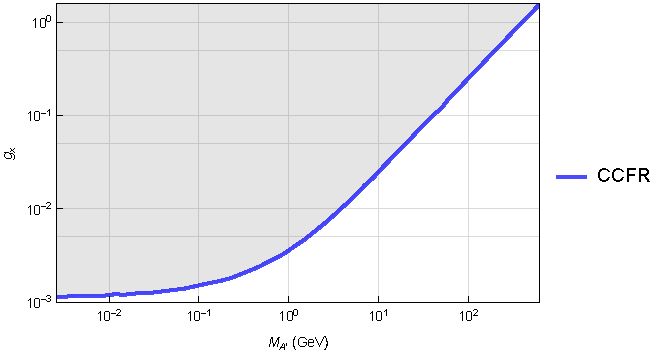
\includegraphics[width=0.6\textwidth]{Constraints picture/ccfr.pdf}
    \caption{Parameter space for the A' boson. The light grey area is excluded at 95\% C.L. by the CCFR measurement of the neutrino trident cross-section.}
    \label{fig:ccfr}
\end{figure}

\begin{figure}[htbp]
    \centering
    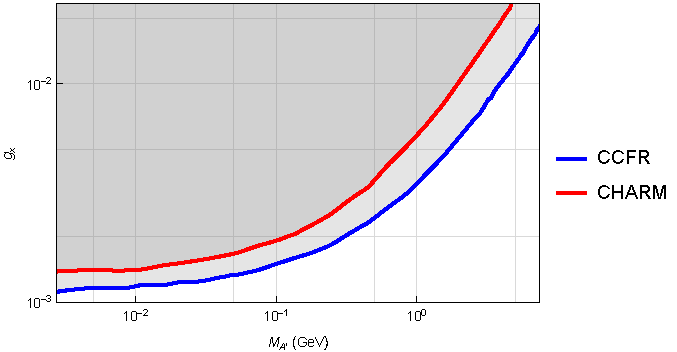
\includegraphics[width=0.6\textwidth]{Constraints picture/lowmassccfr.pdf}
    \caption{Constraints from CHARM-II and CCFR. focusing on the low mass region.}
    \label{fig:lmccfr}
\end{figure}
%By LiMing

\subsection{Invisible Pion Decays}
\label{subsec:pion-invisible}

Stopped-pion experiments provide an additional low-mass handle on the same axial interaction. Ref.~\cite{Altmannshofer:2026opc} studied the invisible three-body decays
\begin{equation}
\pi^+\to \ell^+\nu_\ell X,\qquad X=s,a,V,
\end{equation}
and recast the PIENU search while projecting the reach of PIONEER. The vector benchmark in that work is
\begin{equation}
\mathcal L_V
=V_\alpha\left[
g_V^{(\pi)}\bar\ell\gamma^\alpha\ell
+g_A^{(\pi)}\bar\ell\gamma^\alpha\gamma_5\ell
+\left(g_V^{(\pi)}-g_A^{(\pi)}\right)
\bar\nu_\ell\gamma^\alpha P_L\nu_\ell
\right].
\label{eq:pion-2601-vector}
\end{equation}
Our muon-sector interaction,
\begin{equation}
\mathcal L_{A'}^\mu
=-g_XA'_\alpha\bar\mu\gamma^\alpha\gamma_5\mu
+g_XA'_\alpha\bar\nu_\mu\gamma^\alpha P_L\nu_\mu ,
\qquad g_X\equiv g_SQ_\ell ,
\label{eq:pion-our-map}
\end{equation}
is therefore obtained from Eq.~\eqref{eq:pion-2601-vector} by taking
\begin{equation}
g_V^{(\pi)}=0,\qquad g_A^{(\pi)}=-g_X .
\label{eq:pion-coupling-map}
\end{equation}
Since the pion-decay rate depends on \(\left(g_A^{(\pi)}\right)^2\) for the pure-axial case, the sign convention is irrelevant for the PIENU/PIONEER limits. The relevant channel is
\begin{equation}
\pi^+\to\mu^+\nu_\mu A',
\label{eq:pion-muon-channel}
\end{equation}
which is open only for
\begin{equation}
m_{A'}<m_{\pi^+}-m_\mu\simeq33.9~{\rm MeV}.
\label{eq:pion-kinematic-window}
\end{equation}
The electron channel considered in Ref.~\cite{Altmannshofer:2026opc} is absent at tree level in our model, up to the loop-induced kinetic mixing generated by the \(\mu\) and \(\tau\) currents.

For the pure-axial benchmark the normalized differential rate can be written as
\begin{equation}
\frac{d{\rm BR}(\pi^+\to\mu^+\nu_\mu A')}
{{\rm BR}(\pi^+\to\mu^+\nu_\mu)}
=\frac{g_X^2}{2\pi^2}\,
\frac{dE_\mu dE_{A'}}{m_\pi^2}\,
\frac{F_A(E_\mu,E_{A'};m_{A'})}{(1-x_\mu)^2},
\label{eq:pion-axial-spectrum}
\end{equation}
where \(x_\mu=m_\mu^2/m_\pi^2\), and \(F_A\) is the axial-vector kinematic function given by the \(\left(g_A^{(\pi)}\right)^2\) term of Eq.~(3.10) in Ref.~\cite{Altmannshofer:2026opc}. This spectrum distorts the low-energy tail of the muon kinetic-energy distribution rather than producing a narrow line. Consequently, the bound is obtained by fitting a continuous signal shape to the PIENU muon-energy spectrum, and the projected PIONEER reach follows from the much larger stopped-pion sample and improved target reconstruction.

The invisible-search interpretation is well motivated in our axial \(L_\mu-L_\tau\) realization. For \(m_{A'}<2m_\mu\), the tree-level charged muon mode is closed, while the neutrino modes remain open. Including both \(\nu_\mu\) and \(\nu_\tau\) final states,
\begin{equation}
\Gamma(A'\to\nu\bar\nu)\simeq \frac{g_X^2m_{A'}}{12\pi}.
\label{eq:ap-neutrino-width}
\end{equation}
The loop-induced kinetic mixing opens \(A'\to e^+e^-\) above threshold, but in the minimal \(L_\mu-L_\tau\)-like setup this branching ratio is suppressed by a loop factor and the invisible width dominates across the pion-decay mass window. Thus the invisible \(X\) assumption of Ref.~\cite{Altmannshofer:2026opc} is a good approximation for the parameter space considered here.


Using their recast directly with the above coupling map, present PIENU data exclude roughly \(g_X\gtrsim{\rm few}\times10^{-3}\) at MeV masses, weakening to \(\mathcal O(10^{-1})\) as \(m_{A'}\) approaches the pion-decay endpoint. PIONEER can improve the coupling reach by about an order of magnitude, probing \(g_X\sim5\times10^{-4}\) for \(m_{A'}\sim1~{\rm MeV}\), \(g_X\sim{\rm few}\times10^{-3}\) around \(10~{\rm MeV}\), and \(g_X\sim{\rm few}\times10^{-2}\) around \(20~{\rm MeV}\). In the minimal pure-axial model the muon anomalous magnetic moment gives a much stronger constraint, because the axial vector contributes negatively and has a longitudinal enhancement at low mediator mass. However, if the scalar sector discussed above is arranged to compensate the \((g-2)_\mu\) contribution, pion invisible searches become a useful independent probe. They are most competitive with trident production only at the very low end of the mass window, \(m_{A'}\lesssim{\rm few}\) MeV; for \(m_{A'}\gtrsim10~{\rm MeV}\), the CCFR trident bound is typically stronger.

%By LiMing

\begin{figure}[htbp]
    \centering
    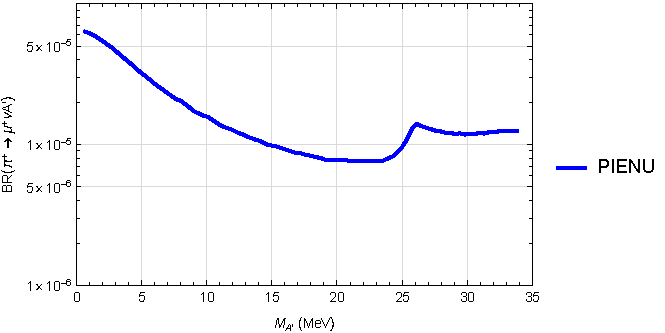
\includegraphics[width=0.6\textwidth]{Constraints picture/πdecayBRConstraints.pdf}
    \caption{Recasted PIENU limits to the $\pi^{+}\to \mu^{+}\nu_{\mu}A'$ branching ratio for axival vector model.}
    \label{fig:pibr}
\end{figure}

\begin{figure}[htbp]
    \centering
    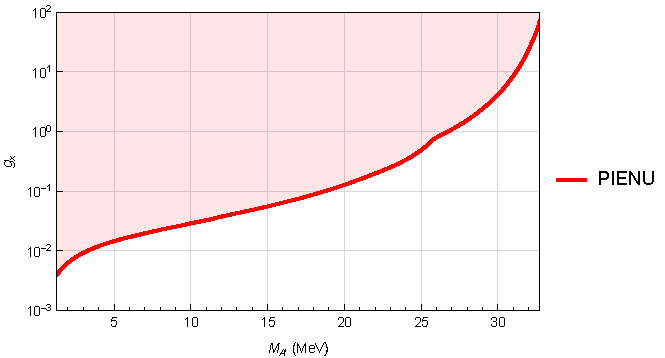
\includegraphics[width=0.6\textwidth]{Constraints picture/πdecayCoupling.pdf}
    \caption{Limits on the couplings of axival vector particles to muons as a function of their mass.}
    \label{fig:picoupling}
\end{figure}

%By LiMing

\subsection{Muon Beam-Dump Searches}
\label{subsec:muon-beam-dump}

Muon beam-dump experiments provide a direct probe of the charged-muon interaction, complementary to neutrino trident production. Ref.~\cite{Chakraborty:2025jbd} studied the present and future sensitivity of NA64$_\mu$, M$^3$, MuSIC, and a future muon beam dump to a \(U(1)_{L_\mu-L_\tau}\) gauge boson. The production process is
\begin{equation}
\mu^- N\to \mu^-N A',
\end{equation}
with the new vector emitted from the incoming or outgoing muon line. Their general improved-Weizsacker-Williams formula already allows independent vector and axial couplings. For our model one simply takes
\begin{equation}
C_V=0,\qquad C_A=g_X,\qquad M=m_{A'} ,
\label{eq:beamdump-map}
\end{equation}
whereas the ordinary four-dimensional \(L_\mu-L_\tau\) benchmark corresponds to \(C_V=g'\), \(C_A=0\).

Keeping the muon mass terms, the axial part of the bremsstrahlung spectrum is
\begin{align}
\frac{d\sigma_A}{dx}
&=
\frac{\alpha^2\chi\,\beta\,g_X^2\,x}
{3\pi m_{A'}^2\left[m_{A'}^2(1-x)+m_\mu^2x^2\right]^2}
\notag\\
&\quad\times
\left[
6m_\mu^4x^4
-2m_{A'}^4(x-1)\{x(x-3)+3\}
+m_\mu^2m_{A'}^2x^2(x-4)(3x-4)
\right],
\label{eq:beamdump-axial-spectrum}
\end{align}
where \(x=E_{A'}/E_\mu\), \(\chi\) is the effective photon flux of the target, and \(\beta\) is the final-state velocity factor. The vector expression used in Ref.~\cite{Chakraborty:2025jbd} is recovered by replacing the square bracket in Eq.~\eqref{eq:beamdump-axial-spectrum} with
\begin{equation}
m_{A'}^2\left[
m_\mu^2x^2\{x(3x-4)+4\}
-2m_{A'}^2(x-1)\{x(x-3)+3\}
\right].
\label{eq:beamdump-vector-bracket}
\end{equation}
Thus the axial and vector production rates coincide only in the formal \(m_\mu\to0\) limit. At low \(m_{A'}\), the nonconservation of the axial current enhances longitudinal \(A'\) emission, and the production rate scales roughly like \(m_\mu^2/m_{A'}^2\) relative to the vector benchmark.

For the invisible NA64$_\mu$ and M$^3$ searches the recast is particularly clean below the dimuon threshold. In this region the tree-level charged-muon mode is closed and Eq.~\eqref{eq:ap-neutrino-width} gives \({\rm BR}(A'\to\nu\bar\nu)\simeq1\). We therefore rescale the four-dimensional single-mode limits of Ref.~\cite{Chakraborty:2025jbd} as
\begin{equation}
g_X^{\rm lim}(m_{A'})
=g_{\rm vec}^{\rm lim}(m_{A'})
\left[
\frac{\sigma_V(g'=1)}{\sigma_A(g_X=1)}
\right]^{1/2},
\label{eq:beamdump-rescale}
\end{equation}
using the same missing-energy cut \(x>0.5\) in the rate ratio. The result is shown in Fig.~\ref{fig:NA64mu}. Since the curves from Ref.~\cite{Chakraborty:2025jbd} are digitized from their \(n_{\rm KKmax}=1\), \(\epsilon_4=\widetilde y_{\rm SM}=0\) figure and then rescaled only at the production-rate level, the plot should be read as an order-of-magnitude phenomenological projection rather than as an official experimental limit. A robust contour would require the experiment-specific target geometry, missing-energy acceptance, finite-lifetime effects, detector response, digitization uncertainty, and the range of validity of the improved Weizsacker-Williams approximation to be propagated together. Representative projected sensitivities in this simplified recast are
\begin{align}
g_X^{\rm NA64_\mu~future}
&\lesssim 4.8\times10^{-8},\,4.9\times10^{-7},\,4.9\times10^{-6}
\quad{\rm for}\quad
m_{A'}=1,\,10,\,100~{\rm MeV},\nonumber\\
g_X^{M^3~{\rm phase~II}}
&\lesssim 3.0\times10^{-8},\,2.4\times10^{-7},\,2.2\times10^{-6}
\quad{\rm for}\quad
m_{A'}=1,\,10,\,100~{\rm MeV}.
\label{eq:beamdump-numbers}
\end{align}
These very strong low-mass numbers reflect the same longitudinal enhancement that also makes the minimal axial-vector contribution to \((g-2)_\mu\) dangerous. We therefore use them only as a guide to the potential reach of muon missing-energy experiments, not as precision exclusions.

%By LiMing
NA64$\mu$

The expected number of signal events corresponding to invisible decays of the form $A' \to \nu\bar{\nu}$ at the NA64$\mu$  experiment is given by Ref.~\cite{111}:
\begin{equation}
N_{\text{signal}} = \frac{N_{\text{MOT}} n_{\text{Pb}}}{\langle dE_\mu/dy \rangle} \int_{E_{\mu,\min}}^{E_{\mu,\max}} dE_0 \int_{x_{\min}}^{x_{\max}} dx \frac{d\sigma_{2\to3}^{A'}}{dx} Br(A' \to \bar{\nu}\nu) N(m_{A'}),
\label{eq:NA64Signal}
\end{equation}

where $d\sigma_{2\to3}^{A'}/dx$ and $Br(Z'\to\bar{\nu}\nu)$ represent the differential cross section and the branching ratio for the event. $N_{\text{MOT}}$ is the total number of muons on target, and $n_{\text{Pb}} = 3.3 \times 10^{22}~\text{cm}^{-3}$ ~\cite{111} denotes the number density of lead nuclei in the target. The quantity $\langle dE_\mu/dy\rangle$ represents the average energy loss per unit length for muons traversing the lead target.

For rescaling, we let 
\begin{equation}
g_X^{\rm lim}(m_{A'})
=g_{\rm vec}^{\rm lim}(m_{A'})
\left[
\frac{\mathrm{N}_{\text{signal} V}(g'=1)}{\mathrm{N}_{\text{signal} A}(g_X=1)}
\right]^{1/2},
\label{eq:beamdump-rescale1}
\end{equation}

\begin{figure}[htbp]
    \centering
    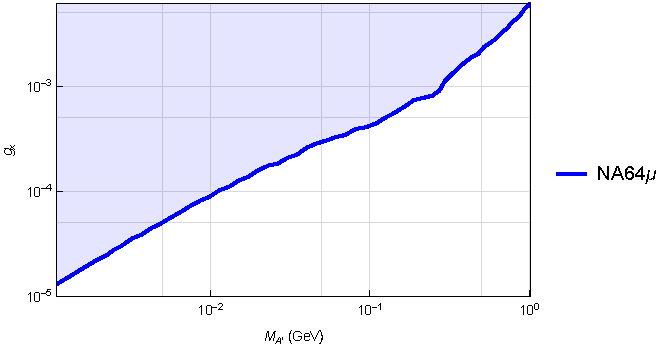
\includegraphics[width=0.6\textwidth]{Constraints picture/NA64mu.pdf}
    \caption{Constraints from NA64$\mu$}
    \label{fig:NA64mu}
\end{figure}

%By LiMing


\subsection{Muon $g-2$}
The muon anomalous magnetic moment is a particularly sharp diagnostic of the Lorentz structure of the new force. The current experimental world average, dominated by the final Fermilab E989 result, is \(a_\mu^{\rm exp}=116592071.5(14.5)\times10^{-11}\). Using the 2025 Muon \(g-2\) Theory Initiative Standard-Model update gives \(\Delta a_\mu\equiv a_\mu^{\rm exp}-a_\mu^{\rm SM} =38(63)\times10^{-11}\)~\cite{Muong-2:2025xyk,Aliberti:2025beg}. This is no longer a robust positive anomaly in the same sense as the older data-driven WP20 comparison~\cite{Aoyama:2020ynm}; therefore we use \((g-2)_\mu\) mainly as a consistency constraint on the axial model.

For a neutral spin-one boson with
\begin{equation}
\mathcal L\supset
A'_\alpha\bar\mu\gamma^\alpha
\left(g_\mu^V-g_\mu^A\gamma_5\right)\mu ,
\end{equation}
the standard one-loop result can be written as~\cite{Leveille:1977rc,Davoudiasl:2014kua,Anastasopoulos:2022ywj}
\begin{equation}
\Delta a_\mu^{A'}=
\frac{m_\mu^2}{4\pi^2m_{A'}^2}
\left[
(g_\mu^V)^2F_V(r)
-(g_\mu^A)^2F_A(r)
\right],
\qquad
r\equiv \frac{m_\mu^2}{m_{A'}^2},
\label{eq:gminus2-vector-axial}
\end{equation}
where
\begin{equation}
F_V(r)=\int_0^1 dx\,
\frac{x^2(1-x)}{1-x+r x^2},
\qquad
F_A(r)=\int_0^1 dx\,
\frac{x(1-x)(4-x)+2r x^3}{1-x+r x^2}.
\label{eq:gminus2-FV-FA}
\end{equation}
The relative minus sign is the main difference from a vector \(L_\mu-L_\tau\) gauge boson. In the heavy-mediator limit,
\begin{equation}
\Delta a_\mu^{A'}\simeq
\frac{m_\mu^2}{12\pi^2m_{A'}^2}
\left[(g_\mu^V)^2-5(g_\mu^A)^2\right],
\qquad m_{A'}\gg m_\mu ,
\label{eq:gminus2-heavy-limit}
\end{equation}
whereas for a light mediator the vector contribution approaches the Schwinger form \(+(g_\mu^V)^2/(8\pi^2)\), while the axial contribution is enhanced by the longitudinal polarization,
\begin{equation}
\Delta a_\mu^{A'}\simeq
\frac{(g_\mu^V)^2}{8\pi^2}
-\frac{(g_\mu^A)^2}{4\pi^2}\frac{m_\mu^2}{m_{A'}^2},
\qquad m_{A'}\ll m_\mu .
\label{eq:gminus2-light-limit}
\end{equation}
In the light-muon mass eigenstate of Eq.~\eqref{eq:light-muon-Apr}, \(g_\mu^V=g_X\sin^2\theta_R\) and \(|g_\mu^A|=g_X\cos^2\theta_R\). Thus the model is dominantly axial and \(\Delta a_\mu^{A'}<0\). If no other new particle contributes, the 2025 comparison roughly requires
\begin{equation}
\Delta a_\mu^{A'} \gtrsim -8.8\times10^{-10}
\quad (2\sigma,\ {\rm WP25}),
\label{eq:gminus2-rough-bound}
\end{equation}
which, in the light-mediator limit, implies the useful estimate
\begin{equation}
g_X\cos^2\theta_R
\lesssim
1.9\times10^{-4}
\left(\frac{m_{A'}}{m_\mu}\right).
\label{eq:gminus2-light-bound}
\end{equation}
This explains why the pure-axial \((g-2)_\mu\) contour in the low-mass region is much stronger than the corresponding vector \(L_\mu-L_\tau\) contour.


%By LiMing
Results: All constraints

\begin{figure}[htbp]
    \centering
    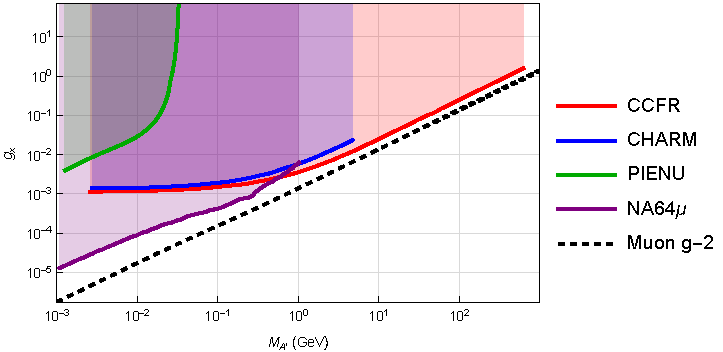
\includegraphics[width=0.6\textwidth]{Constraints picture/AxialConstraints.pdf}
    \caption{Constraints for axial vector model}
    \label{fig:allconstraints}
\end{figure}

%By LiMing

\zb{\subsection{Solar neutrino}

As the axial vector field $A'$ also couples to left-handed neutrinos. The muon- and tau-neutrino currents can also act as source of $A'$~\cite{Fang:2025fvo}. The resulting background field can influence the observed results of the Muon $g-2$ experiment, which enable the current $(g-2)_\mu$ measurement result to be used to constrain the coupling strength. 

We consider solar neutrinos as the dominant source, since they provide the largest neutrino flux at the detector location. The muon- and tau-neutrino components arise through neutrino oscillations during propagation from the Sun to the Earth.
In the relativistic limit, the axial-vector interaction to left-hand neutrinos effectively reduces to a vector-like interaction, such that the neutrino current acts as an electromagnetic-like source which generate a Yukawa potential.
Then, the potential is given by~\cite{Fang:2025fvo},
\begin{equation}
A'^{\alpha} (\vec{x}_d)= \int d^3 x \sum_{\ell = e, \mu, \tau} g_S Q_\ell { \Phi_{\nu_\ell}^{\alpha}(x) }\frac{1}{4 \pi \Delta r}  e^{-m_{A'} \Delta r},
\label{eq:axial-vector-potential}
\end{equation}
where $x_d$ is the position of the detector. $\Phi_{\nu_\ell}^{\alpha}$ is the current of the neutrino $\nu_\ell$, and $\Delta r = |\vec{x}_d - \vec{x}|$ is the distance between the detector and the source. The induced field gives rise to a characteristic sign-changing signal: it is positive during the daytime and negative during the nighttime, superimposed on a small time-independent offset.

In the regime where the interaction range $m^{-1}_{A'}$ is larger than the distance between Sun and Earth, the potential approaches that of a massless mediator, leading to the constraint~\cite{Fang:2025fvo}
\begin{equation}
g_S < 5.8 \times 10^{-18}\  (\text{massless limit}). 
\end{equation}
For larger mediator masses ($m_{A'} > 10^{-17}$ eV), the potential scales as $m^{-2}_{A'}$. The corresponding constraint becomes~\cite{Fang:2025fvo}
\begin{equation}
g_S < 3.1 \times   \frac{ m_{A'}}{{\rm eV}}\ (m_{A'} > 10^{-17}\ \rm{eV}). 
\end{equation}




}

\subsection{Future Muon-Collider Angular Probe}
\label{subsec:muon-collider-angular}

A high-energy muon collider would probe the same muon-philic force in a very different mass range. Ref.~\cite{Huang:2021nkl} studied the ordinary vector \(L_\mu-L_\tau\) gauge boson at a benchmark \(\sqrt{s}=3~{\rm TeV}\) muon collider, using both the two-body process \(\mu^+\mu^-\to\ell^+\ell^-\) and radiative return \(\mu^+\mu^-\to\gamma Z'\). The radiative-return channel is an efficient resonance search for \(m_{A'}<\sqrt{s}\), and in the ultra-relativistic limit its inclusive rate is only mildly sensitive to whether the charged-lepton current is vector or axial. The sharper discriminator for our model is instead the angular distribution in
\begin{equation}
\mu^+\mu^-\to\tau^+\tau^- ,
\end{equation}
where the interference with \(\gamma\) and \(Z\) exchange is chirality dependent.

Neglecting external lepton masses, the unpolarized differential cross section can be written in terms of chiral amplitudes as
\begin{align}
\frac{d\sigma}{d\cos\theta}
&=
\frac{s}{128\pi}
\bigg[
\left(|\mathcal A_{LL}|^2+|\mathcal A_{RR}|^2\right)(1+\cos\theta)^2
\notag\\
&\hspace{2.2cm}
+
\left(|\mathcal A_{LR}|^2+|\mathcal A_{RL}|^2\right)(1-\cos\theta)^2
\bigg],
\label{eq:mucollider-chiral-xsec}
\end{align}
with
\begin{equation}
\mathcal A_{ij}
=
\frac{e^2}{s}
+\frac{g_i^Zg_j^Z}{s-m_Z^2+i m_Z\Gamma_Z}
+\frac{g_i^\mu g_j^\tau}{s-m_{A'}^2+i m_{A'}\Gamma_{A'}} ,
\qquad i,j=L,R .
\label{eq:mucollider-chiral-amplitude}
\end{equation}
For comparison, the ordinary vector and our axial charge assignments are
\begin{equation}
\begin{array}{c|cccc}
&g_L^\mu&g_R^\mu&g_L^\tau&g_R^\tau\\ \hline
{\rm vector} & g'&g'&-g'&-g'\\
{\rm axial} & g_X&-g_X&-g_X&g_X
\end{array}.
\label{eq:mucollider-chiral-couplings}
\end{equation}
This immediately explains why a total-rate reinterpretation of the vector analysis does not capture the main axial effect. Up to a common propagator factor, the photon-\(A'\) interference behaves as
\begin{equation}
\delta_{\gamma A'}^{\rm vector}\propto
-\left[(1+\cos\theta)^2+(1-\cos\theta)^2\right],
\qquad
\delta_{\gamma A'}^{\rm axial}\propto
-(1+\cos\theta)^2+(1-\cos\theta)^2 .
\label{eq:mucollider-interference-pattern}
\end{equation}
The vector case mainly changes the parity-even rate, while the axial case mainly gives a forward--backward distortion. We therefore characterize the effect with
\begin{equation}
A_{\rm FB}=
\frac{\sigma(\cos\theta>0)-\sigma(\cos\theta<0)}
{\sigma(\cos\theta>0)+\sigma(\cos\theta<0)} .
\label{eq:mucollider-afb}
\end{equation}

\begin{figure}[t]
\centering
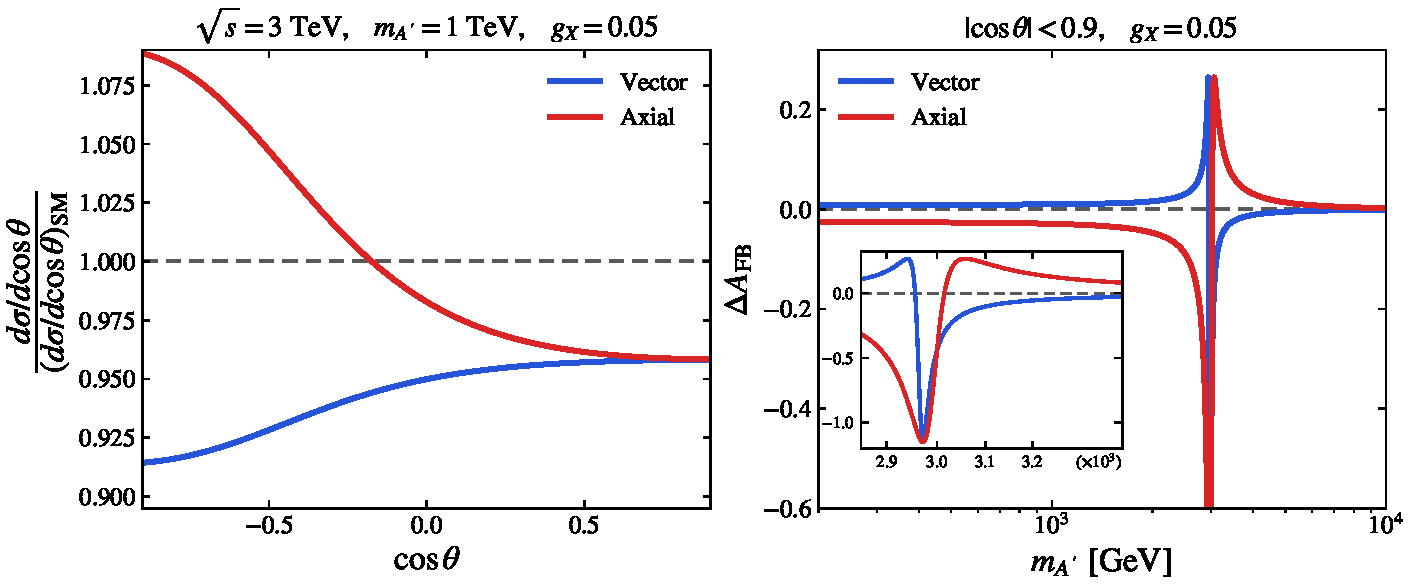
\includegraphics[width=0.94\textwidth]{plots/muon_collider_axial_vector_angular.pdf}
\caption{Future muon-collider angular comparison for \(\mu^+\mu^-\to\tau^+\tau^-\) at \(\sqrt{s}=3~{\rm TeV}\). Left: ratio of the differential cross section to the SM prediction for \(m_{A'}=1~{\rm TeV}\) and \(g'=g_X=0.05\). Right: shift in \(A_{\rm FB}\), integrated over \(|\cos\theta|<0.9\), as a function of \(m_{A'}\). The calculation uses the massless chiral-amplitude formula in Eq.~\eqref{eq:mucollider-chiral-xsec}; the sharp structure near \(m_{A'}\simeq\sqrt{s}\) is the expected \(s\)-channel resonance region.}
\label{fig:muon-collider-angular}
\end{figure}

Fig.~\ref{fig:muon-collider-angular} illustrates the size of the effect. For \(m_{A'}=1~{\rm TeV}\) and \(g_X=0.05\), the vector benchmark changes the \(|\cos\theta|<0.9\) total rate by about \(5\%\), while the axial benchmark changes it by only about \(2\%\). Conversely, the axial case shifts \(A_{\rm FB}\) by \(\Delta A_{\rm FB}\simeq-2.9\times10^{-2}\), larger than the vector shift in this benchmark. A realistic muon-collider limit would therefore require an angular-bin or asymmetry analysis rather than a simple rescaling of the vector \(L_\mu-L_\tau\) contour. This makes the future collider channel complementary to the low-energy probes above: trident, pion-decay, and beam-dump searches constrain the light mediator, whereas a multi-TeV muon collider would test the heavy axial force through parity-odd angular information.


\section{Flavor violating process: $y_{\mu\tau}\neq 0$}
\label{sec:ymutau-nonzero}

The benchmark analysis above was performed in the technically natural flavor limit \(y_{\mu\tau}=0\). We now briefly describe what changes if the gauge-invariant deformation in Eq.~\eqref{eq:4by4-mass-mutau} is kept. This case should not be viewed as a harmless relabeling of the diagonal model. Once the charged-lepton mass matrix is diagonalized, the flavor-nonuniversal \(A'\), scalar, and electroweak interactions are also rotated, and charged-lepton-flavor-violating observables become part of the leading phenomenology.

It is useful to separate the diagonalization into two conceptually distinct steps. Starting from the gauge basis \(\Psi^{(0)}_{L,R}=(\ell^\mu,E^\mu,\ell^\tau,E^\tau)_{L,R}^{T}\), the first step diagonalizes the two flavor-conserving \(2\times2\) blocks, exactly as in Sec.~\ref{sec:2by2-mass}. We write
\begin{equation}
\Psi^{(0)}_{L,R}=\mathcal{U}_{L,R}\Psi^{(1)}_{L,R},
\qquad
\mathcal{U}_{L,R}=
\begin{pmatrix}
U_{\mu,L,R} & 0\\
0 & U_{\tau,L,R}
\end{pmatrix},
\label{eq:ymutau-first-rotation}
\end{equation}
where
\begin{equation}
U_{\ell,L,R}=
\begin{pmatrix}
\cos\theta_{\ell,L,R} & \sin\theta_{\ell,L,R}\\
-\sin\theta_{\ell,L,R} & \cos\theta_{\ell,L,R}
\end{pmatrix}.
\end{equation}
With these block rotations, the real Dirac mass matrix is brought to the intermediate form \(\mathcal{M}^{(1)}=\mathcal{U}_L^T\mathcal{M}\mathcal{U}_R\). In the notation used by the Mathematica diagonalization,
\begin{equation}
\mathcal{L}_m=-
\begin{pmatrix}
	\overline{\ell^{\mu(1)}_L},  &
	\overline{E^{\mu(1)}_L}, &
	\overline{\ell^{\tau(1)}_L}, &
	\overline{E^{\tau(1)}_L}
\end{pmatrix}
\begin{pmatrix}
	m_{\mu,0} & 0  & m_{\mu\tau} x_{11} & m_{\mu\tau} x_{12} \\
	0 & M_{E\mu,0} & m_{\mu\tau} x_{21} & m_{\mu\tau} x_{22}\\
	m_{\mu\tau} x_{33} & m_{\mu\tau} x_{34} & m_{\tau,0} &0\\
    m_{\mu\tau} x_{43} & m_{\mu\tau} x_{44} &  0 & M_{E\tau,0}
\end{pmatrix}
\begin{pmatrix}
	\ell^{\mu(1)}_R \\
	E^{\mu(1)}_R \\
	\ell^{\tau(1)}_R \\
	E^{\tau(1)}_R \\
\end{pmatrix}
+h.c. .
\label{eq:4by4-mass-mutau-v1}
\end{equation}
where \(m_{\mu\tau}\equiv y_{\mu\tau}v/\sqrt2\). The dimensionless coefficients are fixed by the first-step rotations:
\begin{align}
x_{11}&=c_{\mu L}c_{\tau R},&
x_{12}&=c_{\mu L}s_{\tau R},&
x_{21}&=s_{\mu L}c_{\tau R},&
x_{22}&=s_{\mu L}s_{\tau R},\nonumber\\
x_{33}&=c_{\tau L}c_{\mu R},&
x_{34}&=c_{\tau L}s_{\mu R},&
x_{43}&=s_{\tau L}c_{\mu R},&
x_{44}&=s_{\tau L}s_{\mu R},
\label{eq:ymutau-xij}
\end{align}
with \(c_{\ell L,R}\equiv\cos\theta_{\ell,L,R}\) and \(s_{\ell L,R}\equiv\sin\theta_{\ell,L,R}\).

The second step removes the remaining off-diagonal terms in Eq.~\eqref{eq:4by4-mass-mutau-v1}. In the general case this requires another bi-orthogonal transformation,
\begin{equation}
\Psi^{(1)}_{L,R}=\mathcal{V}_{L,R}\Psi^{(2)}_{L,R},\qquad
\mathcal{V}_L^T\mathcal{M}^{(1)}\mathcal{V}_R
=
{\rm diag}(m_\mu,m_{E\mu},m_\tau,m_{E\tau}) .
\label{eq:ymutau-second-rotation}
\end{equation}
The matrices \(\mathcal{V}_{L}\) and \(\mathcal{V}_{R}\) are close to the identity when \(m_{\mu\tau}\) and the heavy-light mixing angles are small. Keeping only the leading terms in \(m_{\mu\tau}\) and in \(\theta_{\mu/\tau,L,R}\), one has \(x_{11}\simeq x_{33}\simeq1\) and all other \(x_{ij}\) are subleading. The intermediate mass matrix then reduces to the light \(\mu\)--\(\tau\) block
\begin{equation}
\mathcal{L}_m=-
\begin{pmatrix}
	\overline{\ell^{\mu(1)}_L},  &
	\overline{E^{\mu(1)}_L}, &
	\overline{\ell^{\tau(1)}_L}, &
	\overline{E^{\tau(1)}_L}
\end{pmatrix}
\begin{pmatrix}
	m_{\mu,0} & 0  & m_{\mu\tau} & 0\\
	0 & M_{E\mu,0} & 0 & 0\\
	m_{\mu\tau} & 0 & m_{\tau,0} &0\\
    0 & 0 &  0 & M_{E\tau,0}
\end{pmatrix}
\begin{pmatrix}
	\ell^{\mu(1)}_R \\
	E^{\mu(1)}_R \\
	\ell^{\tau(1)}_R \\
	E^{\tau(1)}_R \\
\end{pmatrix}
+h.c. .
\label{eq:4by4-mass-mutau-lightlimit}
\end{equation}
In this leading approximation \(\mathcal{V}_L\simeq\mathcal{V}_R\equiv\mathcal{V}_{\mu\tau}\), with
\begin{equation}
\mathcal{V}_{\mu\tau} \simeq \begin{pmatrix}
	1-\frac{m_{\mu\tau}^2}{2(m_{\mu,0}-m_{\tau,0})^2} & 0 & \frac{m_{\mu\tau} }{m_{\tau,0}-m_{\mu,0}} & 0 \\
	0 & 1  & 0 & 0\\
	-\frac{m_{\mu\tau} }{m_{\tau,0}-m_{\mu,0}}  & 0  & 1-\frac{m_{\mu\tau}^2}{2(m_{\mu,0}-m_{\tau,0})^2} & 0 \\
	0 & 0 &0 &1
\end{pmatrix}
\label{eq:ymutau-V-leading}
\end{equation}
or, equivalently, \(\tan2\theta_{\mu\tau}\simeq2m_{\mu\tau}/(m_{\tau,0}-m_{\mu,0})\). The corresponding masses are
\begin{equation}
\begin{aligned}
m_\mu &\simeq m_{\mu,0}+\frac{m_{\mu\tau}^2}{m_{\mu,0}-m_{\tau,0}},&
m_{E\mu} &\simeq M_{E\mu,0},\\
m_\tau &\simeq m_{\tau,0}+\frac{m_{\mu\tau}^2}{m_{\tau,0}-m_{\mu,0}},&
m_{E\tau} &\simeq M_{E\tau,0}.
\end{aligned}
\label{eq:ymutau-leading-masses}
\end{equation}
If the products \(m_{\mu\tau}\theta_{\mu/\tau,L,R}\) are kept, the heavy-light entries in Eq.~\eqref{eq:4by4-mass-mutau-v1} generate additional \(O(m_{\mu\tau}^2\theta^2/M_E)\) mass shifts and small heavy-light admixtures. In that more accurate treatment \(\mathcal{V}_L\) and \(\mathcal{V}_R\) are obtained by diagonalizing \(\mathcal{M}^{(1)}\mathcal{M}^{(1)T}\) and \(\mathcal{M}^{(1)T}\mathcal{M}^{(1)}\), respectively. The numerical electroweak-precision analysis should use this full bi-orthogonal diagonalization; Eq.~\eqref{eq:ymutau-leading-masses} is only the transparent small-angle limit.

For the phenomenology it is useful to keep the discussion in matrix form. Let
\begin{equation}
\Psi^{(0)}_{L,R}=(\ell^\mu,E^\mu,\ell^\tau,E^\tau)_{L,R}^{T},\qquad
\Psi^{(0)}_{L,R}=W_{L,R}\Psi^{(2)}_{L,R},\qquad
W_{L,R}\equiv\mathcal{U}_{L,R}\mathcal{V}_{L,R},
\end{equation}
where \(\Psi^{(2)}\) denotes the final mass eigenstates. Any gauge-basis interaction matrix \(X_{L,R}\) is then rotated according to
\begin{equation}
X_{L,R}^{\rm mass}=W_{L,R}^\dagger X_{L,R}W_{L,R}.
\label{eq:ymutau-mass-basis-couplings}
\end{equation}
In particular,
\begin{equation}
\mathcal{L}_{A'}=
A'_\rho\,\overline{\Psi^{(2)}_i}\gamma^\rho
\left[(g_X Q_L^{\rm mass})_{ij}P_L+(g_X Q_R^{\rm mass})_{ij}P_R\right]\Psi^{(2)}_j ,
\label{eq:ymutau-aprime-couplings}
\end{equation}
with \(Q_{L,R}^{\rm mass}=W_{L,R}^\dagger Q_{L,R}W_{L,R}\). The light-light entry relevant for charged-lepton flavor violation can therefore be parameterized as
\begin{equation}
\mathcal{L}_{A'}\supset
A'_\rho\,\bar\mu\gamma^\rho
\left(g_{\mu\tau}^{L}P_L+g_{\mu\tau}^{R}P_R\right)\tau
{\rm +h.c.},
\qquad
g_{\mu\tau}^{L,R}\simeq
g_X\left(q_{\tau}^{L,R}-q_{\mu}^{L,R}\right)\theta_{\mu\tau}^{L,R},
\label{eq:ymutau-lfv-aprime}
\end{equation}
where the last expression shows the leading light-light mixing-angle dependence when the vector-like leptons are decoupled. Since the present charge assignment is axial in the charged sector, \(q_\mu^L=-q_\mu^R\) and \(q_\tau^L=-q_\tau^R\). The same rotation also gives off-diagonal scalar and electroweak couplings,
\begin{align}
\mathcal{L}_{h,s}&\supset
-h_a\,\bar\mu\left(Y^{a}_{\mu\tau,L}P_L+Y^{a}_{\mu\tau,R}P_R\right)\tau+{\rm h.c.},
\qquad h_a=h,s,\\
\mathcal{L}_{Z}&\supset
Z_\rho\,\bar\mu\gamma^\rho
\left(g_{Z,\mu\tau}^{L}P_L+g_{Z,\mu\tau}^{R}P_R\right)\tau+{\rm h.c.},
\end{align}
where each coupling is obtained from Eq.~\eqref{eq:ymutau-mass-basis-couplings} with the corresponding gauge-basis Yukawa or electroweak matrix.

The most direct consequence is the two-body decay \(\tau\to\mu A'\), which is well known to be a powerful probe of light flavor-violating vector bosons~\cite{Heeck:2016xkh,Ibarra:2021aon}. Neglecting terms suppressed by \(m_\mu/m_\tau\), its partial width is
\begin{equation}
\Gamma(\tau\to\mu A')\simeq
\frac{m_\tau}{32\pi}
\left(|g_{\mu\tau}^{L}|^2+|g_{\mu\tau}^{R}|^2\right)
\left(1-\frac{m_{A'}^2}{m_\tau^2}\right)^2
\left(2+\frac{m_\tau^2}{m_{A'}^2}\right),
\label{eq:tau-mu-aprime-width}
\end{equation}
valid for \(m_{A'}<m_\tau-m_\mu\). The \(m_\tau^2/m_{A'}^2\) term is the longitudinal-vector contribution; in a complete model it is tied to the same symmetry-breaking sector that generates the charged-lepton masses. Thus a very light \(A'\) requires the full UV completion to remain under perturbative control.

The experimental interpretation depends on the subsequent \(A'\) decay. If \(m_{A'}<2m_\mu\) and no additional electron portal is introduced, \(A'\) dominantly decays invisibly into neutrinos, so the relevant observable is \(\tau\to\mu+\slashed{E}\). Belle II has searched for \(\tau\to\ell\alpha\), where \(\alpha\) is an invisible boson, and this provides an important template for the required spectral analysis~\cite{Belle-II:2022heu}. If \(2m_\mu<m_{A'}<m_\tau-m_\mu\), the resonant channel
\begin{equation}
{\rm Br}(\tau\to3\mu)\simeq
{\rm Br}(\tau\to\mu A')\,{\rm Br}(A'\to\mu^+\mu^-)
\label{eq:tau-3mu-resonant}
\end{equation}
must be compared with the \(\tau\to3\ell\) searches~\cite{Belle:2010jhm,Belle-II:2024ami}. Away from the on-shell region one should use the full three-body amplitude
\begin{equation}
\mathcal{M}_{3\mu}=
\frac{
\left[\bar u(p_1)\gamma_\rho(g_{\mu\tau}^{L}P_L+g_{\mu\tau}^{R}P_R)u(p_\tau)\right]
\left[\bar u(p_2)\gamma^\rho(g_{\mu\mu}^{L}P_L+g_{\mu\mu}^{R}P_R)v(p_3)\right]}
{q^2-m_{A'}^2+i m_{A'}\Gamma_{A'}}
-(p_1\leftrightarrow p_2),
\label{eq:tau-3mu-amplitude}
\end{equation}
where the second term accounts for the two identical \(\mu^-\) in the final state.

The two-body expression above can be turned into a useful existing-limit map with minimal additional assumptions. Defining
\begin{equation}
g_{\mu\tau}^{\rm eff}\equiv
\sqrt{|g_{\mu\tau}^{L}|^2+|g_{\mu\tau}^{R}|^2},
\qquad
K_\tau(m_{A'})\equiv
\frac{m_\tau}{32\pi\Gamma_\tau}
\left(1-\frac{m_{A'}^2}{m_\tau^2}\right)^2
\left(2+\frac{m_\tau^2}{m_{A'}^2}\right),
\label{eq:lfv-gtau-def}
\end{equation}
Eq.~\eqref{eq:tau-mu-aprime-width} gives
\begin{equation}
{\rm Br}(\tau\to\mu A')\simeq
K_\tau(m_{A'})\,(g_{\mu\tau}^{\rm eff})^2 .
\label{eq:lfv-two-body-branching}
\end{equation}
For the pure axial benchmark with no electron portal, the relevant \(A'\) branching fractions below the tau threshold are approximately
\begin{align}
{\rm Br}_{\mu\mu}(m_{A'})
&\simeq
\frac{\beta_\mu^3\,\Theta(m_{A'}-2m_\mu)}
{1+\beta_\mu^3\,\Theta(m_{A'}-2m_\mu)},&
{\rm Br}_{\rm inv}(m_{A'})
&\simeq
\frac{1}
{1+\beta_\mu^3\,\Theta(m_{A'}-2m_\mu)},
\label{eq:aprime-lfv-branching-fractions}
\end{align}
where \(\beta_\mu=\sqrt{1-4m_\mu^2/m_{A'}^2}\). The Belle II search for \(\tau\to\mu\alpha\) reports 95\% CL limits on \({\rm Br}(\tau\to\mu\alpha)/{\rm Br}(\tau\to\mu\nu\nu)\) in the range \((0.7-12.2)\times10^{-3}\) for \(m_\alpha<1.6~{\rm GeV}\)~\cite{Belle-II:2022heu}. Treating this as a spectral-template constraint on the invisible vector mode gives
\begin{equation}
g_{\mu\tau}^{\rm eff}
\lesssim
\left[
\frac{{\rm Br}^{95}_{\mu+{\rm inv}}}
{K_\tau(m_{A'})\,{\rm Br}_{\rm inv}(m_{A'})}
\right]^{1/2}.
\label{eq:lfv-invisible-limit}
\end{equation}
Similarly, the latest Belle II limit \({\rm Br}(\tau\to\mu^-\mu^+\mu^-)<1.9\times10^{-8}\) at 90\% CL~\cite{Belle-II:2024ami} implies, in the on-shell region \(2m_\mu<m_{A'}<m_\tau-m_\mu\),
\begin{equation}
g_{\mu\tau}^{\rm eff}
\lesssim
\left[
\frac{{\rm Br}^{90}_{3\mu}}
{K_\tau(m_{A'})\,{\rm Br}_{\mu\mu}(m_{A'})}
\right]^{1/2}.
\label{eq:lfv-3mu-limit}
\end{equation}
The resulting illustrative constraints are shown in Fig.~\ref{fig:lfv-tau-aprime-constraints}. The blue band reflects the published range of the Belle II \(\tau\to\mu\alpha\) limit rather than a point-by-point digitization, and the red curve assumes a prompt on-shell \(A'\to\mu^+\mu^-\) decay. Both curves should therefore be read as a compact guide to the size of allowed \(g_{\mu\tau}^{\rm eff}\), not as a detector-level recast.

\begin{figure}[t]
\centering
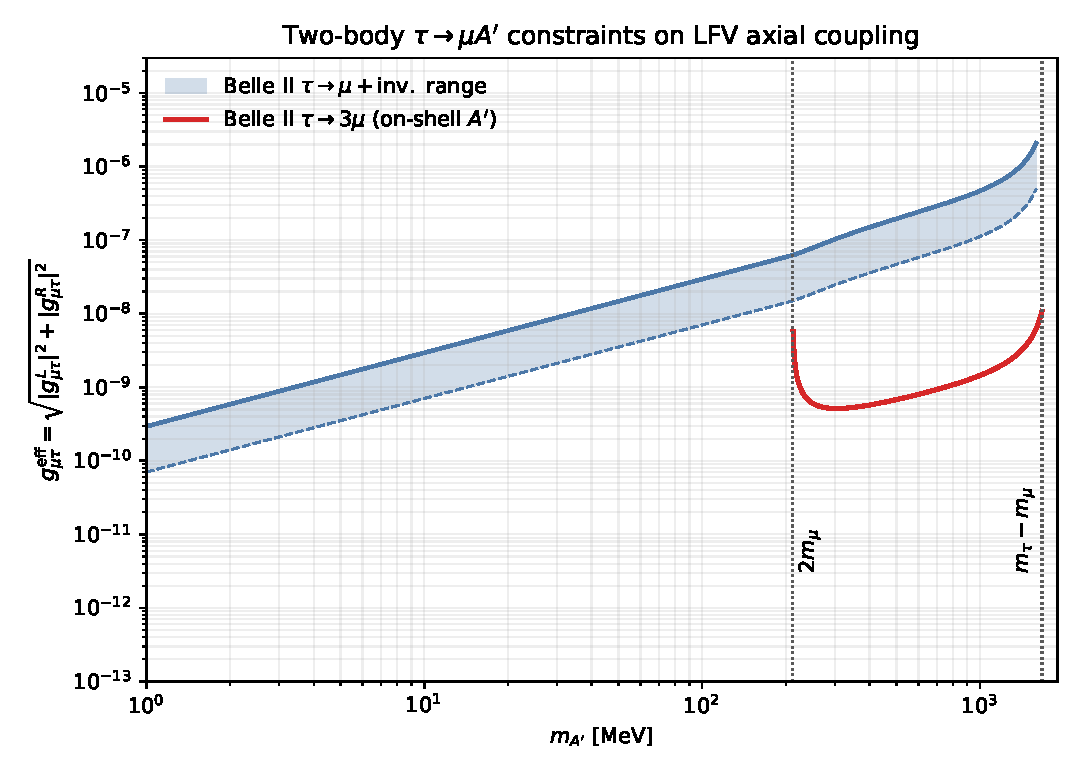
\includegraphics[width=0.78\textwidth]{plots/lfv_tau_aprime_constraints.pdf}
\caption{Existing tau-decay constraints on the effective LFV coupling \(g_{\mu\tau}^{\rm eff}\). The blue band is obtained from the published Belle II range for \({\rm Br}(\tau\to\mu\alpha)/{\rm Br}(\tau\to\mu\nu\nu)\), interpreted as an invisible two-body \(A'\) template. The red curve uses the Belle II \(\tau\to3\mu\) limit in the resonant region \(2m_\mu<m_{A'}<m_\tau-m_\mu\), with the axial threshold factor in Eq.~\eqref{eq:aprime-lfv-branching-fractions}.}
\label{fig:lfv-tau-aprime-constraints}
\end{figure}

Loop-induced and scalar observables are also unavoidable. The dipole operator
\begin{equation}
\mathcal{L}_{\rm dipole}=
\frac{e m_\tau}{2}\,
\bar\mu\sigma^{\alpha\beta}
\left(A_LP_L+A_RP_R\right)\tau F_{\alpha\beta}
{\rm +h.c.}
\end{equation}
gives
\begin{equation}
\Gamma(\tau\to\mu\gamma)=
\frac{\alpha_{\rm em}m_\tau^5}{4}
\left(|A_L|^2+|A_R|^2\right),
\label{eq:tau-mu-gamma-width}
\end{equation}
and must include \(A'\), scalar, and vector-like-lepton loops in the full model. The current Belle bound gives
\begin{equation}
\sqrt{|A_L|^2+|A_R|^2}
\lesssim 1.7\times10^{-9}\ {\rm GeV}^{-2},
\label{eq:tau-mu-gamma-dipole-bound}
\end{equation}
using \({\rm Br}(\tau\to\mu\gamma)<4.2\times10^{-8}\) at 90\% CL~\cite{Belle:2021ysv}. Flavor-violating scalar couplings lead to
\begin{equation}
\Gamma(h\to\mu\tau)\simeq
\frac{m_h}{8\pi}
\left(|Y^{h}_{\mu\tau,L}|^2+|Y^{h}_{\mu\tau,R}|^2\right),
\label{eq:h-mutau-width}
\end{equation}
up to negligible charged-lepton mass corrections. CMS gives \({\rm Br}(h\to\mu\tau)<0.15\%\), or
\begin{equation}
\sqrt{|Y^{h}_{\mu\tau,L}|^2+|Y^{h}_{\mu\tau,R}|^2}
\lesssim 1.1\times10^{-3},
\label{eq:h-mutau-yukawa-bound}
\end{equation}
at 95\% CL~\cite{Harnik:2012pb,CMS:2021rsq}. If the singlet-like scalar satisfies \(m_s<m_\tau-m_\mu\), the analogous \(\tau\to\mu s\) channel should be included as well.

Finally, the same rotations perturb the electroweak currents. Off-diagonal \(Z\mu\tau\) couplings give
\begin{equation}
\Gamma(Z\to\mu^\pm\tau^\mp)\simeq
\frac{m_Z}{24\pi}
\left(|g_{Z,\mu\tau}^{L}|^2+|g_{Z,\mu\tau}^{R}|^2\right),
\label{eq:z-mutau-width}
\end{equation}
while the diagonal entries modify \(Z\mu\mu\), \(Z\tau\tau\), \(W\mu\nu\), and \(W\tau\nu\). ATLAS sets \({\rm Br}(Z\to\mu\tau)<6.5\times10^{-6}\) at 95\% CL after combining the relevant channels~\cite{ATLAS:2021bdj}, corresponding approximately to
\begin{equation}
\sqrt{|g_{Z,\mu\tau}^{L}|^2+|g_{Z,\mu\tau}^{R}|^2}
\lesssim 3.7\times10^{-3}.
\label{eq:z-mutau-coupling-bound}
\end{equation}
These effects are naturally suppressed in the large-\(M_E\) limit, but they provide useful consistency checks together with lepton-universality ratios in tau and \(W\) decays. A systematic treatment of charged-lepton flavor violation in the tau sector is reviewed in Ref.~\cite{Banerjee:2022xuw}. For the present paper we therefore keep \(y_{\mu\tau}=0\) as the benchmark and regard the observables above as the minimal checklist for a future flavor-violating extension.

\section{conclusion}

In this



\bibliographystyle{apsrev4-1}
\bibliography{references}

\end{document}
